\documentclass{article}
\usepackage{mathrsfs}
\usepackage{harpoon}
\usepackage{comment}
%\usepackage{ctex}
\usepackage{color}
\usepackage{amsmath}
\usepackage{mathtools}
\usepackage{simplewick} 
\usepackage{graphicx} % added for subfig
\usepackage{subfigure} % added for subfig
\title{Note for g.s. fit}
\author{Min-Huan Chu and Jinchen He}
\date{}
\usepackage[a4paper,left=20mm,right=20mm,top=20mm,bottom=20mm]{geometry}
\begin{document}
\maketitle
%\tableofcontents
%\pagebreak[4]
\section{Choice of fit method}

\subsection{Fit function}
In the two-state fit method, we did joint fit with three parts: local matrix element $C(z=0, t)$, real and imag part of ratio $\frac{C(z, t)}{C(z=0, t)}$. 
\begin{enumerate}
    \item For local part
    \[ C_2(z=0, t) = c e^{-E_{0} t}\left(1+a_{1} e^{-\Delta E t}\right) \]
    \item For real/imag part of ratio
    \[ \frac{C_2(z, t)}{C_2(z=0, t)} = \frac{\phi_{2}\left(1+b_{1 (re/im)} e^{-\Delta E t}\right)}{1+a_{1} e^{-\Delta E t}} \]
\end{enumerate}

In the 1-state fit method, we fit real/imag part of ratio directly,
\[ \frac{C_2(z, t)}{C_2(z=0, t)} = \phi_{2 (re/im)} \]

1-state fit v.s. two-state fit, which shoule we choose in the analysis of two point data? Two figures are helpful before we set about doing fits:

\begin{enumerate}
    \item Effective mass plot of local matrix element.
    \[ \ln(\frac{C_2(z=0, t)}{C_2(z=0, t+1)}) = E_0 + \ln(1 + a_1 e^{-\Delta E t}) - \ln(1 + a_1 e^{-\Delta E t - \Delta E}) \]
    Therefore, if the effective mass plot is horizontal without decay behavior through t-axis, it is impossible to extract excited state contamination successfully.
    \item Effective mass plot of non-local matrix element.
    
\end{enumerate}

Only when both plots above show the decay behavior, two-state fit is suggested to be tried. Both the coefficient and the effective energy of excited states contamination should be fitted to non-zero results, so that we can claim the two-state fit is successful.


%%%%%%%%%%%%%%%%%%%%%%%%%%%%%%%%%%%%
%%%%%%%%%%%%%%%%%%%%%%%%%%%%%%%%%%%%
\subsection{Example 1}
\begin{figure}[htbp]
    \centering
    \subfigure[Local matrix element]{
    \begin{minipage}[t]{0.5\linewidth}
    \centering
    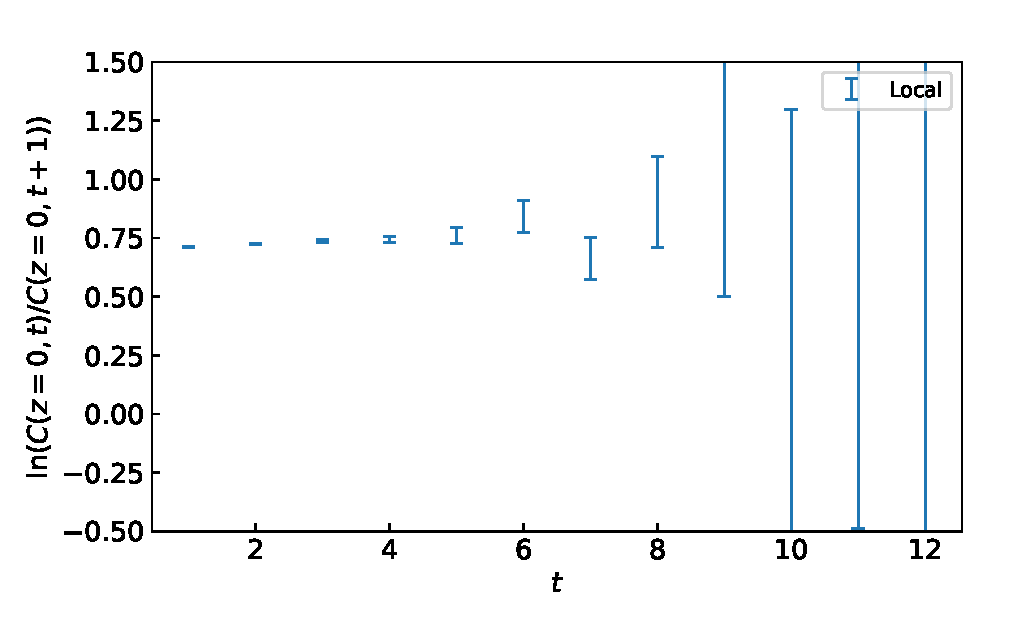
\includegraphics[width=3.2in]{fit_fig/b_local_meff.pdf}
    %\caption{fig1}
    \end{minipage}%
    }%
    \subfigure[Non-local matrix element]{
    \begin{minipage}[t]{0.5\linewidth}
    \centering
    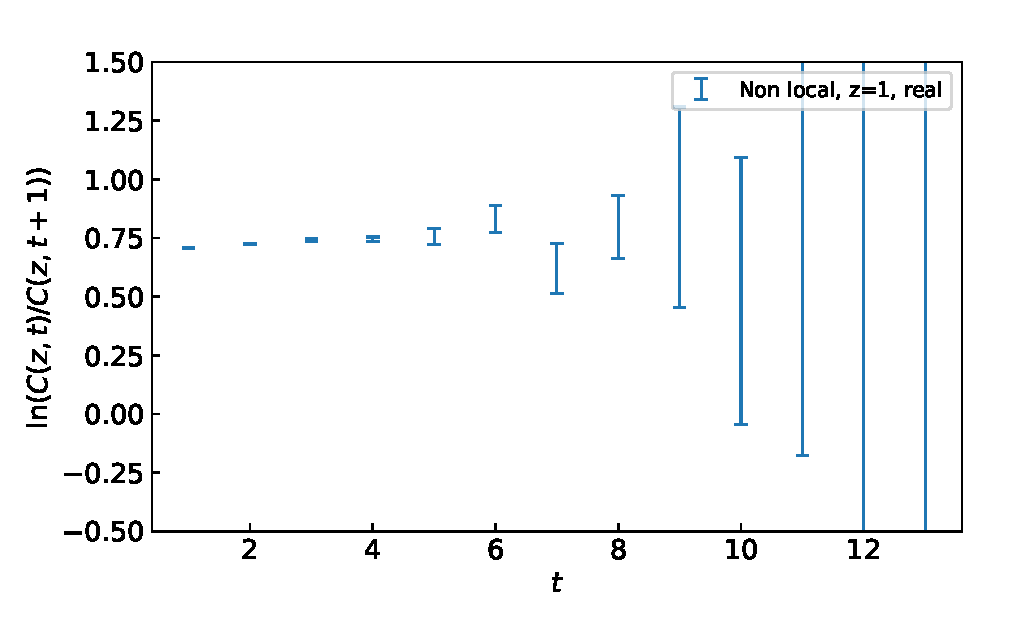
\includegraphics[width=3.2in]{fit_fig/b_non_local_meff.pdf}
    %\caption{fig2}
    \end{minipage}%
    }%
    \centering
    \caption{Effective mass}
\end{figure}

Neither of two plots of effective mass in the Figure.1 shows the exponential decay behavior at small t region, so the 1-state fit method is suggested.

\begin{figure}
    \centering
    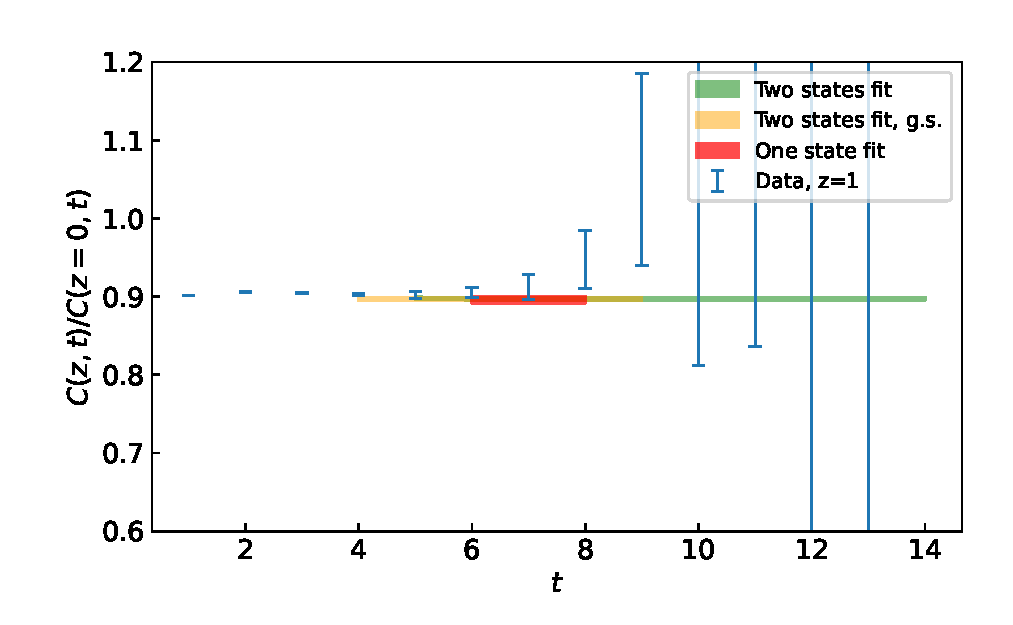
\includegraphics[height=7cm,width=11.3cm]{fit_fig/b_fit_result.pdf}
    \caption{Fit result comparison}
\end{figure}

This is the output of two-state fit,
\begin{equation}
    \begin{aligned}
    &\text { Least Square Fit: } \\
    &\text { chi2/dof [dof] }=0.91[18] \quad Q=0.57 \quad \log G B F=96.901 \\
    &\text { Parameters: } \\
    &\text { $g.s._{re}$ } \quad 0.8964 (25) \\
    &\text { $a1$ } \quad -2.6 (6.5) \\
    &\text { $b1_{re}$ } \quad -1.6 (4.1) \\
    &\text { $dE1$ } \quad 1.30 (73) \\
    &\text { $E0$ } \quad 0.7442 (82)
    \end{aligned}
\end{equation}

From the output it can be found that the fit result of excited state's coefficient $b_1$ covers zero within the error, which means the two-state fit failed to extract the excited state contamination.






%%%%%%%%%%%%%%%%%%%%%%%%%%%%%%%%%%%%
%%%%%%%%%%%%%%%%%%%%%%%%%%%%%%%%%%%%
\subsection{Example 2}

\begin{figure}[htbp]
    \centering
    \subfigure[Local matrix element]{
    \begin{minipage}[t]{0.5\linewidth}
    \centering
    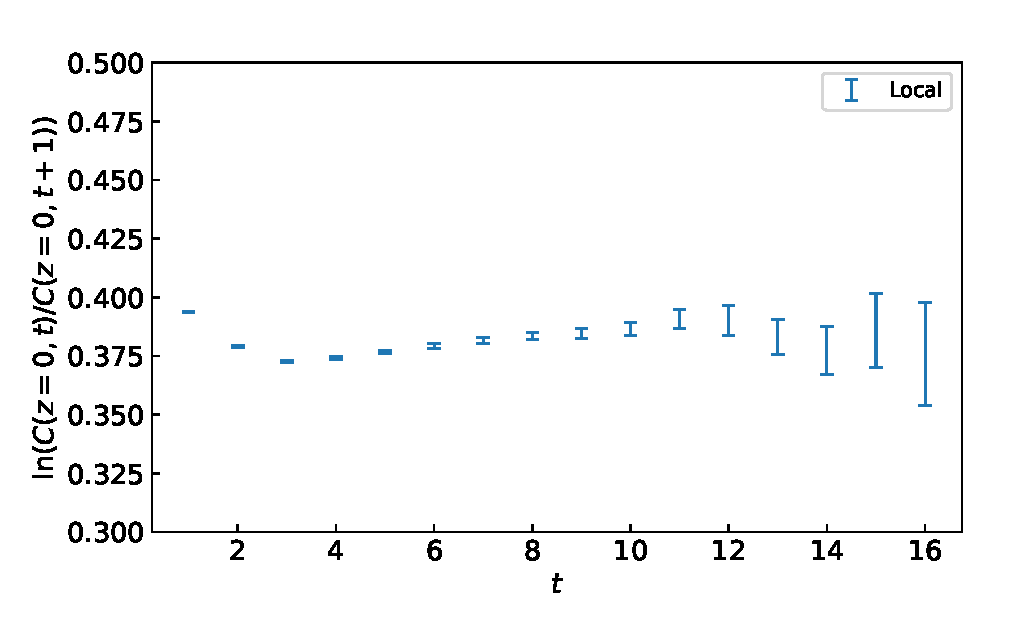
\includegraphics[width=3.2in]{fit_fig/g_local_meff.pdf}
    %\caption{fig1}
    \end{minipage}%
    }%
    \subfigure[Non-local matrix element]{
    \begin{minipage}[t]{0.5\linewidth}
    \centering
    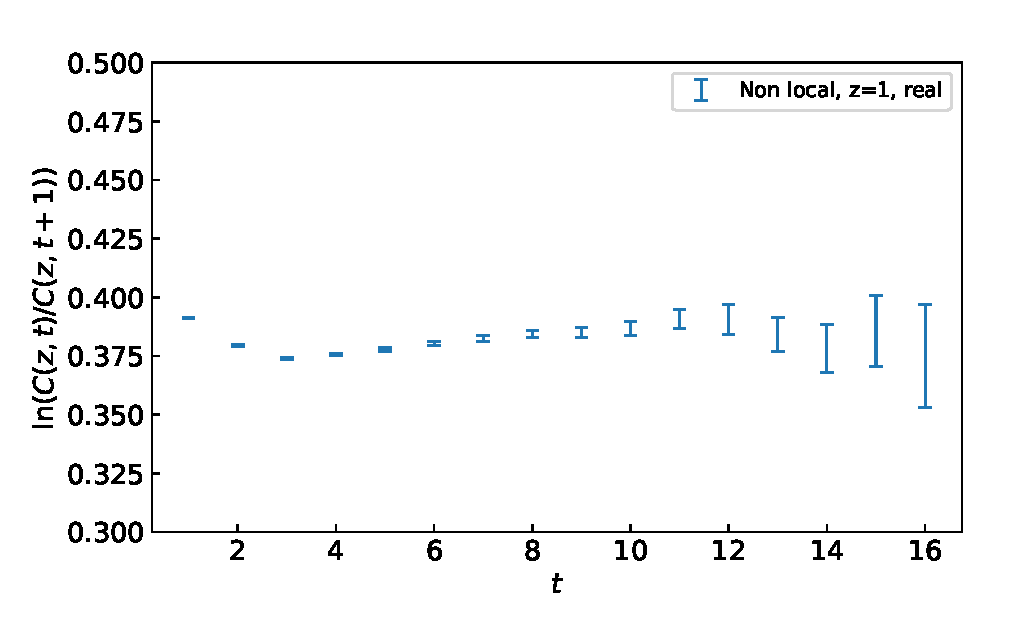
\includegraphics[width=3.2in]{fit_fig/g_non_local_meff.pdf}
    %\caption{fig2}
    \end{minipage}%
    }%
    \centering
    \caption{Effective mass}
\end{figure}

Both of two plots of effective mass in the Figure.3 shows the exponential decay behavior at small t region, so the two-state fit is worthy to try.

\begin{figure}
    \centering
    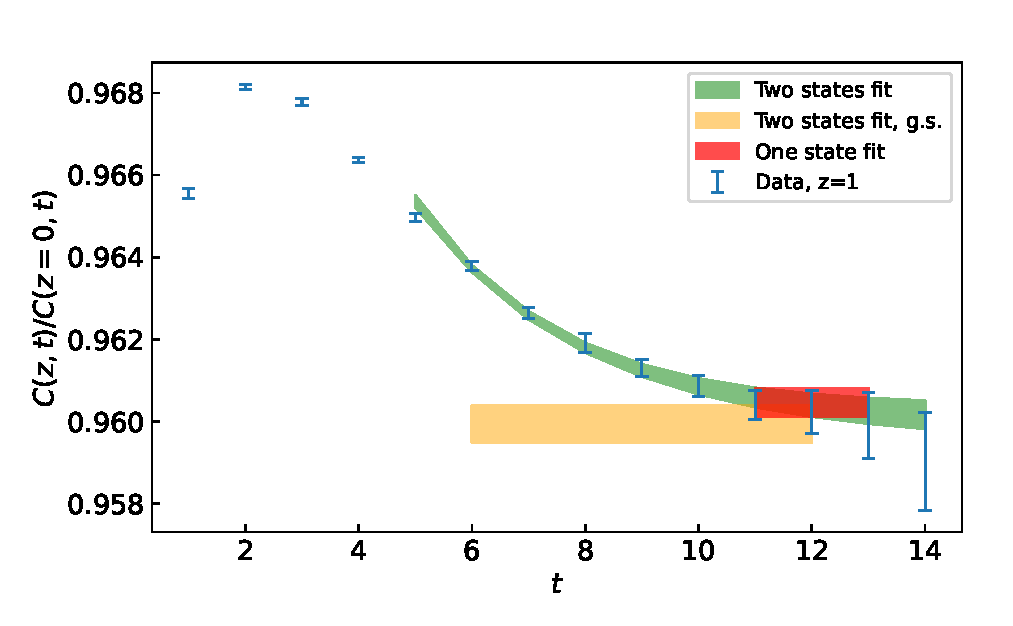
\includegraphics[height=7cm,width=11.3cm]{fit_fig/g_fit_result.pdf}
    \caption{Fit result comparison}
\end{figure}

This is the output of two-state fit,
\begin{equation}
    \begin{aligned}
    &\text { Least Square Fit: } \\
    &\text { chi2/dof [dof] }=0.2[21] \quad Q=1 \quad \log G B F=194.25 \\
    &\text { Parameters: } \\
    &\text { $g.s._{re}$ } \quad 0.95954 (56) \\
    &\text { $a1$ } \quad -0.231 (41) \\
    &\text { $b1_{re}$ } \quad -0.206 (40) \\
    &\text { $dE1$ } \quad 0.294 (53) \\
    &\text { $E0$ } \quad 0.3899 (20)
    \end{aligned}
\end{equation}

From the output it can be found that the fit result of excited state's energy $\Delta E$ and coefficient $b_1$ does not cover zero within the error, which means the two-state fit succeeded to extract the excited state contamination.

\section{Factors affecting fit method}
\subsection{Source for generating data}
In generating the two point function data $C_2(z,t)$, there're two sources, wall source and point source. 

For wall source, the definition can be written
\begin{displaymath}S_{wall}(x,t,\vec{P}_s)=\sum_{\vec{x}_0}e^{-i\vec{P}_s\vec{x}_0}\delta^3(\vec{x}-\vec{x}_0)\end{displaymath} 
In the sum of space variable $x_0$, the excited states offset each other, causing it hard to determine the excited energy $\Delta E$ in local $C_2(z=0,t)$
\begin{displaymath}C_2(z=0,t)=ce^{-E_0t}(1+a_1e^{-\Delta Et})\end{displaymath}

For point source, the definition turns to
\begin{displaymath}S_{point}(x,t,\vec{P}_s)=e^{-i\vec{P}_s\vec{x}_0}\delta^3(\vec{x}-\vec{x}_0)\end{displaymath} 
there's not this effect, thus it is easier to determine the excited energy $\Delta E$ in local $C_2(z=0,t)$.

\subsection{Hadron mass}
If the excited energy is very close to ground state, the meson mass of $C_2(z=0,t)$, obviously, the two-state fit can not work well.
\begin{displaymath}C_2(z=0,t)=ce^{-E_0t}(1+a_1e^{-\Delta Et})\end{displaymath}
In another word, the first term in the right side hardly dominate when $\Delta E\sim 0$.

We have investigate three cases $\pi(130)$, $\eta_s(670)$, $J/\psi(3000)$ in the same lattice approach, the results are as follows in FIG. {\color{red}(xx).}

{\color{red} Smaller excited state energy should be more suitable for two-state fit, coz the e.s. effects would not be invisible compared with the g.s. }


\subsection{Hadron momentum}
With the same consideration, the hadron momentum also affect two-state fit. Because of the relative size for ground state energy and excited state energy.

{\color{red} Though big momentum will lead to bigger ratio $\frac{E_{g.s.}}{E_{e.s.}}$, or say smaller relative energy gap, but it also means much more significant suppression on $e^{-\Delta E t}$, so we should compare $1$ with $e^{-\Delta E t}$ to say whether there is an obvious t-dependence to do two-state fit. }


For pion two point function at the momentum $P^z=\{0,6,10\}\times\frac{2\pi}{L}$, the following figure shows the two-state fit results. 

\end{document}